
\chapter{系统设计与实现}
\section{设计思路}
\subsection{主要任务}

为了解决现有任务调度控制方法的不人性化和不直观以及拓展更多功能的需求,故提出本项目,旨在为解决以上问题而更近一步。具体任务列举如下:

\begin{itemize}
	\item 通过可视化分析的方法及时地了解到某时间节点下,正常和异常服务器的运行状态参数(CPU利用率、memory利用率、disk利用率等)和服务器本身的各项硬件指标(CPU数目、memory大小等),并且可以进行实时切换的功能;
	\item 通过调度信息(task、job和instance),由图形展示出导致异常的原因归咎于哪个具体task或job,由此得到用户操作对后端服务器的影响;
	\item 直观看到服务器任务(task)、作业(job)和实例(instance)之间的包含关系以及数目大小,得到主要占用服务器资源的作业信息,做出相应调整;
	\item 通过热力图刷新迅速掌握某服务器节点在过去一段时间的工作状态,帮助工作人员寻找规律,辅助其他模块判断异常节点的出错动机;
	\item 了解到在某一时间点下拥有记录的所有服务器节点的运行状态和该时间下运行某任务的服务器异常数目,定位异常高峰,并由此有针对性地确定需要观察的时刻。
\end{itemize}

本文拟根据以上需求设计并实现相应的系统模块,设计和实现过程在本章的余下章节将展开详细说明。

%\newpage
\subsection{关键问题的解决方法}

%\subsubsection{数据处理}
\noindent{\textbf{3.1.2.1\quad 数据处理}}

上文中提到,处理、读取并查找庞大量级的数据文件成为了一大难题。出于对本项目模型性和实时性的考虑,经过团队的讨论最终决定选择八天中第二天的数据作为数据集模拟数据流进行研究。然而问题是经过分割后的数据文件的体积仍然超过了研究地点所有独立设备的内存极限,解决方法在于python对数据处理方法的改变:如算法\ref{alg-1}所示,改变以往的处理中小型数据的思路和方法,将庞大的数据集每次按需读入设备内存进行处理,故得出两种可行的方法,python csv中的按行读取方法和pandas的块级读取的方法,即每次根据电脑内存大小只读取原数据文件的一小部分,等这一部分被处理和计算结束后再去重复操作处理其他部分的数据。这样便实现了任意大小的文件都可以被任意设备进行处理和计算的方法。

\begin{algorithm}
	\caption{Huge data file reade}
	\label{alg-1} 
	\textbf{Input}: data\_path
	
	1:\textbf{initialize}:reader=csvReader(data\_path)
	
	2:\textbf{for} row  \textbf{in} reader do
	
	3:\qquad filter by Conditions
	
	4:\qquad write(row)
	
	5:\textbf{end for}

\end{algorithm}

\noindent{{\textbf{3.1.2.2\quad 集群表示及定位故障源}}}

为了准确而简洁地表示每一个任务所持有的job、task与instance参数,以及如何将三者与具体被调度地服务器节点联系起来,经过讨论拟采用以下方案:采用可是分析展示方法中的tree结构,可以清晰明了地展示三者之间地层次关系。与此同时,在叶子节点的节点处与相应处理服务器绑定,反映正在运行此instance的服务器所处的运行状态。通过以上方法,就完美解决了任务调度信息的层次关系和不同数据文件之间的关联。

\noindent{{\textbf{3.1.2.3\quad 故障域算法}}}

数据集本身有许多参数来说明后端服务器节点的状态。 控制阈值是确定异常域的有效方法,取决于三个有价值的领域:CPU利用率,内存利用率和磁盘利用率。 通过为这三个参数分配权重,系统可以确定节点在处理任务实例时是否处于高负荷。 算法二描述了在我们的研究中识别异常的方法:

$$Value_{hl}=x\cdot\frac{S_{\beta +\gamma}}{S}+y\cdot\frac{S_{\alpha+\gamma}}{S}+z\cdot\frac{S_{\alpha+\beta}}{S}$$

在上面的算法中,$\alpha$,$\beta$和$\gamma$分别代表CPU,内存,磁盘的阈值。 我们使用概率统计学的思想来设置适当的阈值,以保持异常高负荷节点的比例接近10%。 可以像这样计算高负荷的负荷值。

\noindent{{\textbf{3.1.2.4\quad 时序性及空间性}}}

为了将数据可视化与节点状态的时序性结合起来,我们拟通过日历图的热力排布来展示一个服务器节点在过去一段时间内的运行状态。通过像素块颜色的深浅,直观反映某节点的健康程度。

由于缺少节点的地理位置信息,所以不能将集群的地理分布在地图上展示,前期拟定的三维数值坐标展示将只用树状结构叶子节点的热力色块来展示。因为使用者并不用清楚的知道此时此刻服务器的各种利用率参数,只需要知道该节点健康与否即可。

\subsection{技术栈}
$Vue.js+express+python+R+webpack+mongoDB+mongoose+vuex+Promiss+D3.js+
echarts.js+axios+$\LaTeX$ $

\noindent{{\textbf{3.1.3.1\quad 编程工具及设备选择}}}

Visual Studio Code(March 2019 version 1.33)

System:Windows 10  Intel(R) Core(TM) i5-8400 CPU 16.0GB 2.81GHz

\noindent{{\textbf{3.1.3.2\quad 前端框架}}}

根据项目的特点,我们选用vue.js作为用户前端设计和实现的框架,具体的优势如下:
\begin{itemize}
	\item 基于MVVM的双向绑定机制,使开发者在编写前后台参数传递的时候简洁易行,避免了过多的ajax请求来进行组件间与前后台的通讯,加快了用户在操作可视化视图时系统的处理速度;
	\item 拥有很多已整合的辅助模块,比如vue-resource、vuex、vue-d3等,对开发过程尽可能地简化,更有效率的进行数据请求、状态管理和可视化组件的开发;
	\item 还有其他如组件化、渐进式、异步批处理等优势,为节省文章篇幅在此不再赘述。
\end{itemize}

\noindent{{\textbf{3.1.3.3\quad 后端框架}}}

根据项目的特点,采用了node.js的express作为后端框架,主要还是因为其具有如下优势:

\begin{itemize}
	\item Node.js比传统的后台处理语言更加快速,代码更加简洁
	\item 与后台数据库mongoDB的整合更加流畅,请求更加方便
	\item 更活跃的社区支持,使后期调试变得更有效率
\end{itemize}

\noindent{{\textbf{3.1.3.4\quad 数据库}}}

因为系统实现的目标是实时监控服务器集群,所以计划采用后端连接数据库,用来储存数据并返回给后台所请求的数据。由于项目所采用的模拟数据集为csv文件格式,mongoDB将会是我们的首选数据库:其非关系型数据存储格式完美适配原数据文件特点,而且具有弱一致性,对于本项目的可视图形渲染一次请求大量数据的特点,一定程度上保证了处理和刷新视图的速度和用户访问速度。

\noindent{{\textbf{3.1.3.5\quad 可视化框架}}}

在可视分析领域,有非常多种数据可视化的实现方式,类似python、R等在数据处理方面颇有建树的语言都有各自的第三方库来支持数据可视化。但是如果想实现更自由的功能和表达性更强的视图,那最好的方式就是用专业的数据驱动文档语言D3.js来实现,不但拥有更全面灵活的组件、更活跃的社区,还能完美结合现有的BS架构,嵌入到已有的系统中。

\section{模块设计}

基于前端框架vue.js的模块化布局渲染的原则,加上出于未来对功能的拓展和维护有利的考虑,本项目自身将采用模块化开发。每一种不同的功能模块将被设计为不同的组件。各种组件各司其职,互不干扰,通过组件间的通信来实现系统与用户的交互。

与此同时,基于上文对整个系统的构思和对关键问题的分析,将对系统做如下的组件设计:
模块一:在整个系统中,必须含有可以映射整个时间轴的数据总览模块,该模块作为整个用户UI界面的入口模块,是在整个时间线上对所有服务器节点状态的表示。由于拟向使用者展示所有异常服务器的变化趋势,在趋势的表达上,会使用一种折线图的方式来模拟每个时间戳上所含有的所有异常服务器节点的个数。在此组件里,用户可以根据图像所表达的趋势针对特殊时刻或者自己想观察的时刻,来过滤节点,同时根据传递的参数,刷新别的视图,从而达到整个页面的布局响应,即所谓的Level-0层次组件。

模块二:在Level-0级组件的基础上,我们将设计一种渐进式的响应模块Level-1。该类模块是上一层模块的递进,通过使用者对上一层模块的操作,进一步向其展示更加深入的可视化视图。本层级拟设计两个视图,其一是分布式力向(force-directed)布局的树形视图,其二是拥有数量表示的旭日(sunburst)视图。以上是通过对分布式任务调度的具体表达,从而来解释job、task、instance之间的从属关系,从而帮助判断造成异常的用户原因(详细设计将在3.2.1.2中进行阐述)。

模块三:通过对Level-1级视图的操作,进而展示最顶端层级Levl-2。Level-2是Level-1之上更细致更深入的视图层级,可以精确到具体的某个节点,从时序性和空间性两个角度展示其最一段时间的运行状态和相关的运行参数。拟用基于热力像素的日历图(calendar)图来表示某一节点在从现在到过去的状态描述,用直方图(histogram)来展示服务器节点本身的属性和运行参数,从而辅助Level-1层判断该节点的异常类型(详细设计将在3.2.1.3及3.2.1.4中进行阐述)。

\subsection{总览曲线(Level-0)}
\noindent{{\textbf{3.2.2.1\quad 基本设计}}}

基于从时序性的角度展示服务器节点异常个数的总览曲线,将对该视图作如下设计:横轴代表时间(原数据文件time\_stamp字段),纵轴代表该时间点下异常节点的个数(<4000),用曲线的拐点来表示异常个数,然后再将所有的拐点连结起来形成一条无断点的DAG\footnote{Directed Acyclic Graph,指的是一个无回路的有向图。}图形。由原数据集的特征可以得出,横轴的控制范围是(100000,172000)之间,单位为秒,为期一整天的记录;纵轴是(0,4000)之间的异常节点数,随着时间的递进做着规律性变化。

\noindent{{\textbf{3.2.2.2\quad 时序性导致的自变量密集度过高的问题}}}

由于本次项目所取的数据是原数据第二天的记录,时间戳记录从100000到172000,每十秒一个记录,所有对自变量来说有7000余个记录,映射在时间坐标轴上就是7000余个坐标点,远远超过了常规视图中的基数。这就导致了一个问题,当操作者想在一台长1980px的显示设备上看到整个曲线,由于时间点的密集度过高,所呈现出来的视图远远脱离了折线的特征,整条曲线的记录过分重叠,使得人眼无法辨认和映射每个时刻对应的异常节点的个数,更不要说去观察曲线的变化趋势了(如图\ref{pic-1}所示)

\begin{figure}[h]
	\centering
	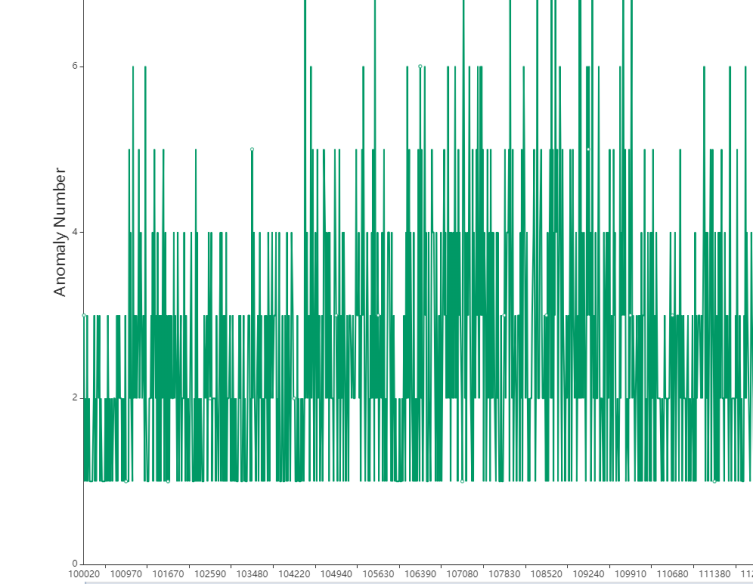
\includegraphics[height=0.5\textwidth]{pic-1}
	\caption{记录过于密集的曲线}
	\label{pic-1}
\end{figure}

为了解决以上问题,经过资料的查阅,拟定出来以下方法来协助我们观察密集度过高的曲线:在时间轴的下方插入一个范围控制条,来控制我们向观察的区域大小。由于我们往往不需要观察所有节点的轨迹,当我们想看到某一小段时间内的折现变化情况,就可以通过改变控制条的长短,来决定视图所要显示的范围大小。

\begin{figure}[h]
	\centering
	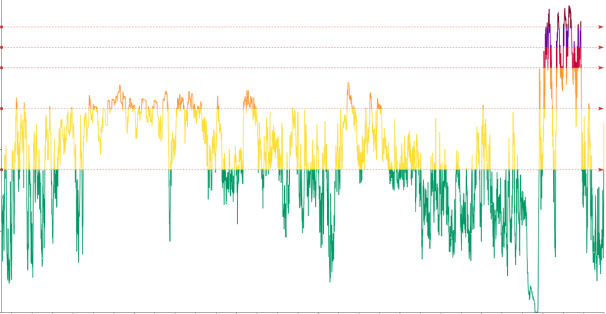
\includegraphics[height=0.4\textwidth]{pic-2}
	\caption{优化后曲线视图}
	\label{pic-2}
\end{figure}

如图\ref{pic-2}所示,通过控制下方控制条的长短,可以有效减小原视图折线的密集度,从而可以很清楚的展示异常节点的数量变化规律,从而帮助操作者更加有效的观察全程的变化趋势从而挑选有研究意义的时刻。

\subsection{节点异常检测(Level-1)}

\noindent{{\textbf{3.2.3.1\quad 基本设计}}}
想要通过视图体现出任务调度中各个层级(job,instance,task)之间的关系,基础元素拟采用树形结构的节点集,一个节点集表示中心父节点job下的task与instance的分布情况,结构示意图如图\ref{pic-3}所示:

\begin{figure}[h]
	\centering
	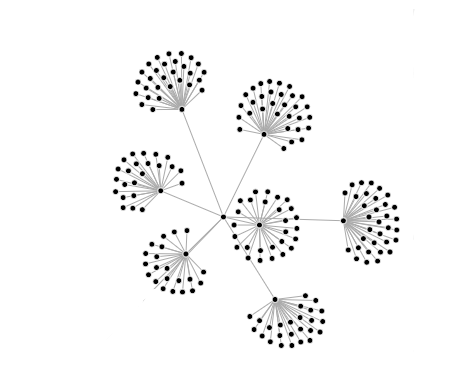
\includegraphics[height=0.4\textwidth]{pic-3}
	\caption{树形节点结构图}
	\label{pic-3}
\end{figure}

我们将基于Level-0组件设计渐进响应组件Level-1。这种类型的模块是前一个模块的渐进模块,并通过用户在前一个模块中的操作进一步显示更详细的图形视图。此级别旨在设计两个视图,其中一个是强制定向布局中的树,另一个是具有强响应函数的旭日形图。所有这些都是通过分布式任务调度的具体表达来解释作业,任务和实例之间的联系,从而有助于确定用户导致负载异常的原因。
异常定位的主要处理模块如图\ref{fig-4}所示。这种节点集分为三个级别。有必要通过视图反映任务调度中每个级别(作业,实例,任务)之间的关系。基本元素旨在采用树结构的节点集,每个集合逻辑地表示中心父节点作业下的任务和实例的分布。为了视图的直观性和后续交互的可操作性,我们将不同层级的节点分别设置参数,以便使用者更好的区分:

\begin{figure}[h]
	\centering
	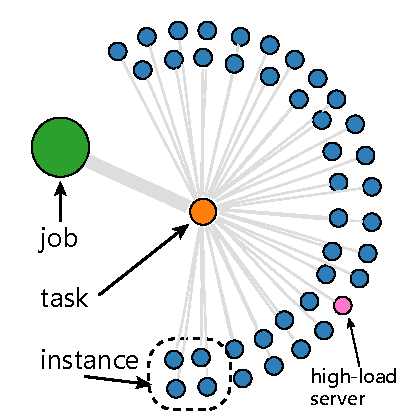
\includegraphics[height=0.4\textwidth]{4}
	\caption{设计展示}
	\label{fig-4}
\end{figure}

job节点的半径为8px,颜色用十六进制表示为:\#2ca02c;

task节点的半径为5px,颜色用十六进制表示为:\#ff7f0e;

instance节点的半径为3px,颜色用十六进制表示为:\#1f77b4。

在此基础上,如果我们想要给视图元素添加与运行insatnce的服务器节点的健康状况,拟定将环绕task的instance节点群增加颜色维度,渲染的色块表示该instance所在服务器的异常与否。这样我们就可以得到任务调度与服务器节点的关系,通过观察异常节点的分布和job簇之间的关系,得到出现异常的原因。

重点是反映视图组件中的异常服务器节点,除了作业调度的显示。 如上面的图2所示,每个任务实例由一个独立的服务器机器独立处理,我们显示处理任务实例的服务器节点的负载级别。 这种方法似乎是随机的,但通过图形方法,操作员可以获得异常服务器节点布局的规律,并进一步了解一些异常作业节点。

\noindent{{\textbf{3.2.3.2\quad 数量级的精确表示}}}

经过以上分析,基本确立了实现系统功能的主视图的设计,虽然在表示上清晰明了,但是其中的元素还缺少一种对任务调度的精确刻画。所以出于功能完整性的考虑,在保留原视图的基础上,增加Level-1层级额外的可视化组件,如图\ref{pic-4}所示:

\begin{figure}[h]
	\centering
	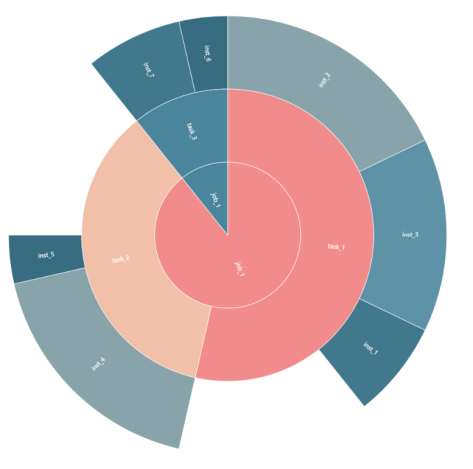
\includegraphics[height=0.4\textwidth]{pic-4}
	\caption{旭日图模型}
	\label{pic-4}
\end{figure}

以上组件在可视分析领域被称作旭日(sunburst)图,在保证了层级关系的基础上,还增加了对节点元信息的描述,比如可以输出原组件不能输出的调度参数的Id信息,每个task所包含instance的数量级以及各层级调度元素占所有元素的占比的多少,并且交互性强,更加全面客观的反映job簇的精确信息。

\subsection{时序性展示(Level-2)}

为了增强时序性的展示,拟加入可以体现过往状态的可视化组件来实现对服务器节点的全面描述。我们挑选日历图(calendar)的原因是其功能和特点完全可以还原原本的设计思路:用横坐标和纵坐标两个维度来表示过去时间的延续性,用中央色块的颜色变化来展示在某一时刻下该节点运行的健康程度。

颜色表示的原理是基于生物学的人体视觉通道,红色的饱和度越大表示该节点在此时的异常程度更低。在时间的表示上,我们以10秒为一个递进单位,来展示服务器节点在某时刻之前1小时之内的所有运行状态,试图从中寻找规律,判断该节点的异常周期或者常规的健康状况。

上面显示的图形方法适用于整个时间线中的所有后端服务器节点。 然而,当操作员想要观察单个节点的状态时,它们似乎并不那么令人信服,并且所谓的1级和2级组件仅在同一时刻说明某个时刻的状态。 我们添加新组件以增强时序描述,并丰富我们从上一层视图中选择的指定异常节点的描述。 我们打算通过加热图描绘过去一段时间内某个服务器的状态,并通过一种直方图显示机器的各种操作参数。 通过热图和直方图的两个组成部分,我们使特殊节点的顺序描述更加全面和详细。

\begin{figure}[h]
	\centering
	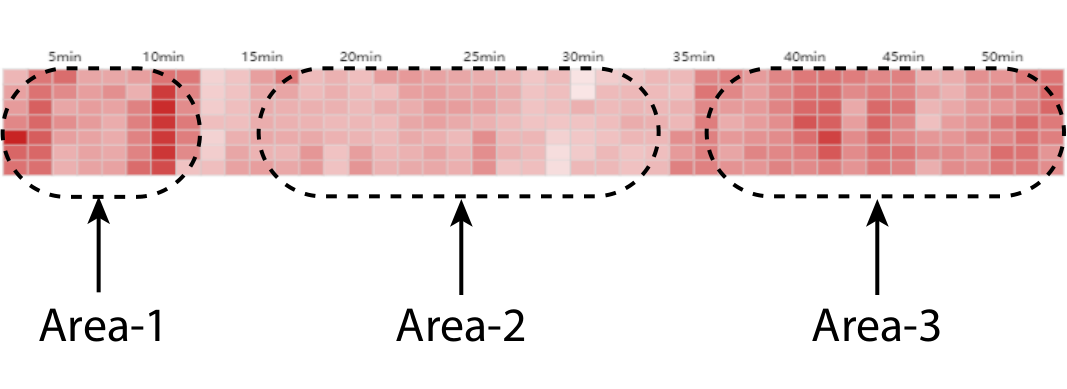
\includegraphics[height=0.3\textwidth]{pic-5}
	\caption{日历图模型}
	\label{fig-5}
\end{figure}

图\ref{fig-5}描述了单独节点状态的变化,颜色块的差异说明了过去60分钟内服务器性能的状态。每个块表示过去一段时间内的10秒的跨度,并且由所有块组成的区域表示一小时的时间线。视图组件通过可视通道的映射在时间上向操作员示出单个服务器节点的性能。具有低饱和度的那些块表示服务器的硬件的良好性能,并且那些深红色的块表示服务器的性能在目前具有高负载值的硬件时并不是那么优越。

例如,图\ref{fig-5}中的Area-1说明了服务器A,例如,在过去的15分钟内处于高负载状态,尤其是在您选择观察之前的大约14分钟内。然后在17分钟之后,服务器运行状态的性能保持在正常水平,如Area-2所示,之后,在Area-3中,服务器以某种方式具有另一个高负载阶段。

此级别的视图组件通过直观的性能抽象增强了特定服务器节点的时间可伸缩性,并使用另一个视图组件直方图增强了节点的详细描述,该直方图将与下一章中的其他模块一起进行分析。

\section{模块实现}
\subsection{客户端与服务端的搭建}

需要先设置整个项目的目录结构,只有完整简洁的项目结构,才能支撑起整个系统错综复杂的请求。整个项目的文件结构如下:

├── build

├── config

├── node\_modules

├── server

│   ├── db\# 数据库连接与配置

│   ├── routes\# 后端路由文件

│   ├── views\# 视图文件

│   └── app.js\#服务器入口文件

├── src

│   ├── App.vue\#视图根节点

│   ├── main.js\#webpack打包入口文件

│   ├── components\# 项目组件

│   ├── router\# 前段路由

│   └── store\# 全局状态管理

├── static\#静态资源

├── index.html\#项目搭载html文件

├── package.json\#配置列表

├── README.md\#项目解释文档

└── 项目日志

\begin{itemize}
	\item “build”和“config”文件夹里存放项目所需要的配置项
	\item “node\_modules”文件夹存放项目所需要的第三方依赖
	\item “server”文件夹存放后台服务端的代码文件
	\item “src”文件夹存放前段客户端的代码文件
	\item “static”存放静态文件和测试数据
\end{itemize}

服务端入口文件为app.js,声明express后端框架,设置本地服务器端口,引入数据库并且发送请求测试后台是否连接成功。配置代码与后端接口页面显示如下:

\begin{lstlisting}[caption=配置前后端服务器,frame=shadowbox,language={java}]
const metaModel = require('../db/model/meta');
const usageModel = require('../db/model/usage');
const resultModel = require('../db/model/result');
const result = require('../db/model/result')

module.exports = function(app){
	app.get('/',function(req,res){
	res.send('Hello,here is /')
});

\end{lstlisting}

\begin{figure}[htb]
	\centering
	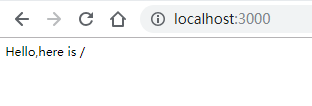
\includegraphics[height=0.2\textwidth]{pic-6}
	\caption{连接成功}
	\label{pic-6}
\end{figure}

图\ref{pic-6}证明后台已经搭建成功,成功向后台返回信息。

在后端搭建成功的基础上,我们将利用vue语法实现第一个前端展示页面:在components中创建模块test.vue(以vue为后缀名的是vue中声明的组件文件),想要在项目结构中调用该文件,必须首先将组件挂载到根节点App.vue中,在再服务端入口文件中引入根节点,在webpack打包后完成对项目结构的封装,即可在前端页面展示

\subsection{总览曲线(Level-0)}

为了达到简洁健壮的动态web设计的要求,实现曲线组件之前需要统筹组件本身与其他模块之间的数据流向工作。设计结果的规划如下:BS架构的前端技术框架为vue.js,在框架中用vue组件的形式去实现可视化曲线的模块,通过异步请求数据向本地服务器端发送数据请求,经过mongoose的查找和筛选之后返回给前台所要求的数据集,再通过d3.js或者echarts.js将数据渲染到前端组件中,即完成了一个可视化模块的实现。

\begin{lstlisting}[caption=挂载服务器app,frame=shadowbox,language={java}]
const express = require('express');

const routers = require('./routes/index.js');
const metaModel = require('./db/model/meta');
const usageModel = require('./db/model/usage');
const resultModel = require('./db/model/result')
require('./db/db');
const app = new express();
routers(app);
app.listen(3000);
\end{lstlisting}

\begin{lstlisting}[caption=测试vue渲染DOM元素,frame=shadowbox,language={java}]
<template>
<div>
<h1>{{message}}</h1>
</div>
</template>

<script>


export default {
data () {
return {
date:'',
message:''
}
},

created(){
let now = new Date();
this.message = `现在的时间是${now}`
}
}
</script>
\end{lstlisting}

\begin{figure}[h]
	\centering
	
\includegraphics[height=0.15\textwidth]{pic-7}
	\caption{测试结果}
	\label{pic-7}
\end{figure}

如图\ref{pic-7}所示,vue组件中的元素已经通过全局引用成功挂载到了服务端。
至此,前后端的搭建工作已经顺利完成,接下来的章节将介绍每个可视分析组件的具体实现过程。

\subsection{分时任务调度展示(Level-1)}
在实现可视化功能之前,需要对数据结构和视图代码做一些准备。设定将渲染曲线的数据集Array设计成二维数组的结构。但由于原数据文件的个体过大,为了优化查找速度,我们将原数据先做一层处理,以得出任务调度的服务器节点的异常情况(用boolean值表示)。

对异常域的判定,我们将采用加权模拟的算法,将整个故障占比稳定在10\%左右,根据对三个关键参数(util\_CPU、util\_memory、util\_disk)的计算,得出判定machine是否异常的布尔值,再对mongoDB数据库表结构加以重构,得出我们将进行进一步统计的数据集。

我们的数据层任务是得到每一个时刻异常服务器节点的总个数,所以还要对数据进行加工。原生JavaScript算法可以实现对目标数据集的聚合,但更有效率的实现方法是利用mongoose的聚合管道,语言优美并且功能性更强大,如关键代码段3.4所示:

\begin{lstlisting}[caption=管道实现聚合查询,frame=shadowbox]
.aggregate([
{$match:{warning:{$eq:1}}},
{$group:{_id:'$time_stamp',warning:{$sum:1}}},
{$sort:{'_id':1}}
])
.then(d=>{
res.json(d)
})
\end{lstlisting}

得到所需要的信息之后,还需要对数据进行重构来匹配可视化组件。在保证处理速度的前提下,这里我们用最经典的js代码来操作并重构数组,得到符合要求的数据集之后,需要我们来编写真正的可视化组件了。在上一章提到过,我们需要加入控制条来对要展示的有效数据进行筛选,从而是整个视图变得更加合理和美观;其次,我们需要加入更多的效果控件来对用户体验进行优化:

\begin{itemize}
	\item 实现鼠标滚轮来带动页面的缩放;
	\item 实现健康状态对应视觉通道的色块图例,以及在视图中根据对数据的绑定来显示颜色分类,增强判别能力;
	\item 实现鼠标hover状态来展示对应的时刻数据以及异常节点个数;
	\item ……
\end{itemize}

时序曲线的实现模块linec,被项目根节点调用并声明,通过webpack打包输出在web浏览器上,效果如图所示:

\begin{figure}[h]
	\centering
	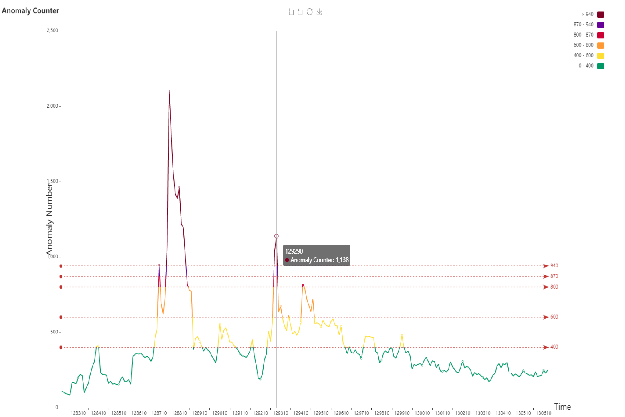
\includegraphics[height=0.6\textwidth]{6}
	\caption{入口视图效果图}
	\label{pic-8}
\end{figure}

如图\ref{pic-8}展示的是在116250时刻到120150时刻的异常节点个数的时序变化,可以看出在图中峰值是119110秒时异常个数最多的2722个,最低的是118380时刻的1084个异常节点数。可见我们的设计对全过程趋势的表达效果良好,每个时刻的状态颜色映射较清晰。

\newpage
\subsection{具体节点参数展示(Level-2)}
\noindent{{\textbf{3.2.3.1\quad 力导向树形图}}}
在输入数据集准备可视化渲染之前,还需要对输入的数据集进行研究。储存在数据库中记录任务调度的原生数据是按条目划分的JSON数组,每一条记录含有inst\_name,task\_name,job\_name等字段名,我们需要将其经过处理最终输出我们可以渲染的形式,实现的算法如下:

\begin{lstlisting}[caption=格式化row data,frame=shadowbox,language={java}]
...
let exist = new Array();
let index = new Array();
let group = new Array();
for(let j in Json){
if(exist.indexOf(Json[j].inst_name )== -1){
index.push(Json[j].inst_name);
group.push(1);
exist.push(Json[j].inst_name);
}
}
...
\end{lstlisting}

如代码段3.5所示,我们将数据处理为单位job簇是具有一个根节点(job)、多个二级子节点(task)和若干个叶子结点(instance)的格式,某一时刻下包含多个job簇,组成在这一时间点下任务调度的可视化视图。展示实现之后的效果图,下图是在时间戳为120010时刻的任务调度可视化分析图:

\begin{figure}[h]
	\centering
	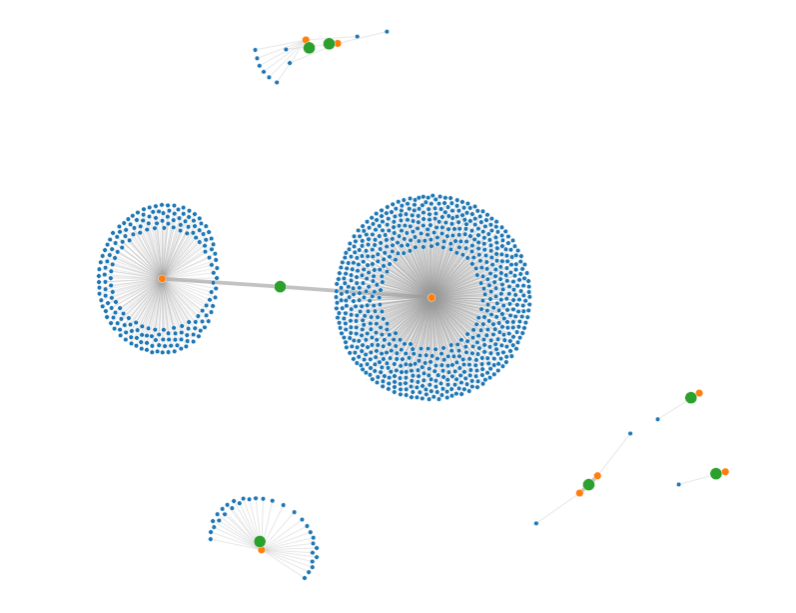
\includegraphics[height=0.45\textwidth]{pic-8}
	\caption{力导向图效果图}
	\label{pic-9}
\end{figure}

如图\ref{pic-9}所示,根据job级节点的渲染格式为\#2ca02c,节点半径最大来观察,得出该时刻共有7个job簇:左下角是job和task数目为1、instance数目为32的节点集合,出于视图中间、体积最大的是有1个job根节点,2个次级task节点和共1851个的instance节点。

整个布局采用力向布局,拥有节点数越多的集合对其他单位的斥力也就越大,这样很好的保证了图形的可观察性和布局的美观,D3.js画布元素选择与力向布局的参数设置的部分代码如图所示:

\begin{lstlisting}[caption=基于D3关于svg图形的实现,frame=shadowbox,language={java}]
d3(){
let svg = d3.select("svg"),
width = +svg.attr("width"),
height = +svg.attr("height");

let color = d3.scaleOrdinal(d3.schemeCategory10);

let simulation = d3.forceSimulation()
.force("link", d3.forceLink().id(function(d) {
return d.id;
}).distance((d)=>{
return d.value == 0.25 ? 70:10;}
))
.force("charge", d3.forceManyBody().strength(-5))
.force("x", d3.forceX())
.force("y", d3.forceY())
.force("center", d3.forceCenter(width / 2, height / 2));
\end{lstlisting}

\noindent{{\textbf{3.2.3.2\quad 节点健康状态的关联查询展示}}}

根据usage数据文件中的warning字段进行关联查询,但是由于D3视图文件和usage文件不再一个表内,而mongoose聚合管道关联查询所得的数据集由于太过庞大超过了后阿提数据接口所能容纳的最大限额,采用经过讨论拟采用以下算法:

\begin{lstlisting}[caption=基于vuex对数据的集中式管理,frame=shadowbox,language={java}]
usageModel
.where('time_stamp').equals(req_time)
.then(response => {

let warningArray = new Array();
for (let i in warningId) {
for (let j in response) {
if (warningId[i][0] == response[j].machine_id) {
let obj = new Object();
...
obj.inst_id = warningId[i][1];
obj.warning = response[j].warning;
warningArray.push(obj)
break
}}}
o.warningArray = warningArray;
res.json(o);
})
...
context.commit('getdata',res.data.result);
context.commit('getarray',res.data.warningArray)
...
\end{lstlisting}

构造数据映射列表使数据在渲染的过程中在内置vuex中检查状态,根据结果对节点颜色进行修改,即可实现节点健康状态的关联展示。

\noindent{{\textbf{3.2.3.3\quad 旭日图}}}

为了增强视图的可表达性和交互的操作性,在保留Level-1级视图中第一组件功能的完备性的前提下,增加另一组件旭日图,来表达关系调度的层级关系和各单位的数量关系。

首先,先设计算法以格式化数据:以d3.js所带的d3.stratify函数对上一节的处理结果进行层次化处理,但由于该函数的机制原则是只能包含一个根节点,所以在数据中先构造一个辅助根节点“origin”,在调用root.descendants()取父节点的所有后代包含关系,再设计算法使得结构型树形结构变为扁平型数据结构。文字描述算法的复杂性略有抽象,下图是该思想的部分实现算法辅助说明:

\begin{lstlisting}[caption=构造父子节点结构数据,frame=shadowbox,language={java}]
let links = linksProcess(a);

let root = d3.stratify()
.id(d => {
return d.target
})
.parentId(d => {
return d.source
})
(links)
let d = root.ancestors()[0].children;;
let data = structure(d)
\end{lstlisting}

所以将每次得到的关系数据集送入该函数群输出结果,再将结果送到已经设计好的d3可视化代码中,即可实现对旭日图的渲染,如图\ref{pic-91}所示:

\begin{figure}[h]
	\centering
	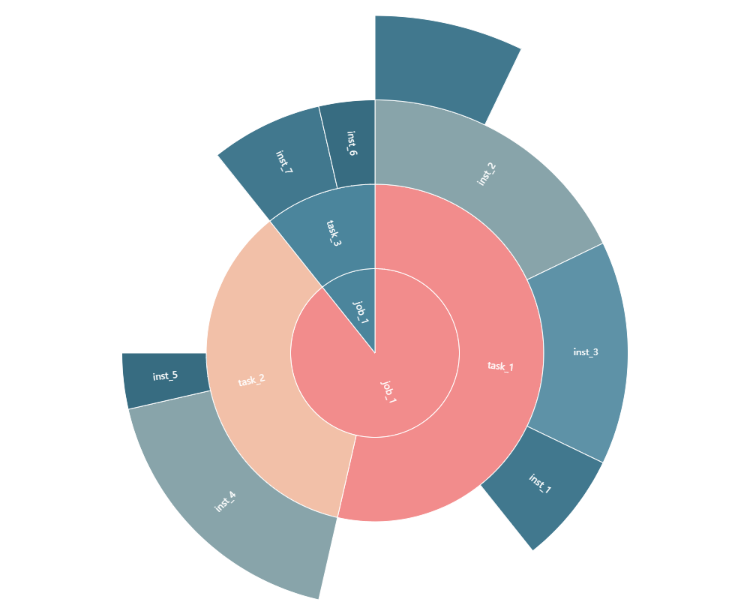
\includegraphics[height=0.45\textwidth]{pic-9}
	\caption{旭日图效果图}
	\label{pic-91}
\end{figure}

从图中即可更有效的了解到instance节点的数目信息,以及显示各个层级元素的具体名称,以便通过交互在Level-2视图中查看。

\newpage
\subsection{时序性展示(Level-2)}

在描述整个调度元素的层级Level-1上,我们增加针对独立服务器节点的表达模块,称作Level-2层级。在Level-2层级上,我们可以更全面系统的看到某个节点的细节信息。

仅仅满足了任务调度的空间性描述还远远不够,如果能在时序性的刻画上帮助使用者了解到服务器节点的过往情况,往往能更加全面的判断节点的故障类型,甚至找出异常性的周期规律。可见,增加视图的时序性是有必要的。

对二维模式(时间-状态)的刻画上,为了符合可视分析原则之一的直观性,我们选择像素排布的模式,对服务器节点所组成的空间阵列,用视觉通道的映射来实现对健康状况的表达。

由于监视器测得的数据的时间间隔是以10秒为一个单位,在10秒级的间隔来说,节点状态的变化往往是趋于线性的,所以我们拟以10秒为刷新单位,将过去1h之内的状态信息渲染于已经设定好的像素中。

根据热力图显示的原理,每一个色块使用基于红色的渲染,用色相的饱和度与色彩的明暗来描述服务器节点的状态,实现视图如下:

\begin{figure}[h]
	\centering
	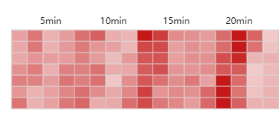
\includegraphics[height=0.2\textwidth]{pic-10}
	\caption{日历图效果图}
	\label{pic-10}
\end{figure}

该模块表示了在0-20min的区间内,服务器节点状态的描述,由图可见,红色越深代表此时该节点的负载越高,红色越浅则表示节点的负载越低,性能越好。色块的布局基于对时间的排布,可见该表示方法对向使用着输出节点状态的时序性的效果还是非常好的。

\subsection{交互实现}
为了增强系统的交互性,优化使用者的用户体验和加强整个系统的功能性,我们拟将更多的交互手段加入系统,让使用者可以通过对其中一个组件的操作,来带动全部组件的刷新效果,使所有组件之间更具有整体性。这时便突出了之前我们使用Level来定义组件层级的逻辑价值。

如我们在上文计划的那样,最基础的逻辑层Level-1,是整个系统的入口元素,也是我们进行用户操作的最初始的元素,通过该组件的特点,使得我们对全局的把控更加具有针对性,所以Level-0层级组件也适合作为入口元素关联其他组件来实现视图的联动效果。

众所周知实现组件之间的传值是一件非常繁琐的工作。在vue中需要不断地调用props来对你要传递的参数进行操作,而且针对于本次项目组件之间的关联度非常大的情况下,这种方法在后期调试和维护时难度将会非常的大。在这种需求的驱动下,我们计划将采用vuex来实现对全局状态的管理和维护。

由于篇幅原因不再过多解释vuex的概念及其工作原理,将直接说明其调用的过程。首先在原曲线组件代码中增添点击事件,事件中全局调用vuex,将vuex.\$store.state的time\_stamp值更新为点击元素的params。在状态管理层的state层级实现的代码结构如下:

\begin{lstlisting}[caption=state层级结构,frame=shadowbox,language={java}]
let state = {
time_stamp:'',
data:[],
counter:0,
warningArray:[]
};
\end{lstlisting}

在mutations实现的代码结构如下:

\newpage
\begin{lstlisting}[caption=mutations层级结构,frame=shadowbox,language={java}]
let mutations = {

submitTime(state,name){
state.time_stamp = name
},
getdata(state,d){
state.data = d;
},
getarray(state,d){
state.warningArray = d;
}
};
\end{lstlisting}

在actions实现的代码结构如下:

\begin{lstlisting}[caption=actions层级结构,frame=shadowbox,language={java}]
let actions = {
getData(context,d){
context.commit('submitTime',d);
Vue.http.get(`/result?name=${d}`)
.then(res=>{

context.commit('getdata',res.data.result);
context.commit('getarray',res.data.warningArray)
});
}
};
\end{lstlisting}

以上代码的区别在于,state是全局状态变量声明,而mutations是对state进行操作的控件,而actions中含有各种异步操作。所以在点击事件触发后,是利用axios向后端数据接口发起数据请求,将时间参数通过axios传递到后台,在后台进行mongoose的数据处理过程,然后将处理得到的结果输出到接口,再通过vuex调用mutations控件改变全局data数组的值,即可实现对state的更新,以便其他所有vue组件在需要时通过this.\$store.state.data来调用全局状态state。

实现了这种功能之后,在组件中对全局状态的渲染也就水到聚成了。通过监听函数watch()来对state的刷新保持监听模式,一旦数据发生更新,便触发对可视化模块的重新渲染以达到刷新的效果。

通过全局状态管理模式的另外一个好处就是,所需要被渲染的数据经过点击只需要请求和发送一次,在其他组件请求的过程中,不需要再发送axios请求,而是直接使用vuex的全局状态来保持对视图的更新。在一定程度上优化了视图的处理速度,对这种一次请求1M以上数据对数据请求要求十分高效的项目来说,这种改变是有必要的。

\section{性能测试与评估}

为了证明我们研究的可行性,我们基于数据集cluster-trace-v2018模拟了实际环境中的使用和操作。

数据集对于我们的模拟很有价值,因为数据集是从实际的分布式系统操作中跟踪和获得的。 为了证明我们研究的可行性和有效性,我们从我们使用的过程中选择了一个典型且令人信服的案例。 图\ref{fig-6}是Level-1视图组件的示例,其描绘了在时间戳114550处的作业调度的实际情况。

\begin{figure}[h]
	\centering
	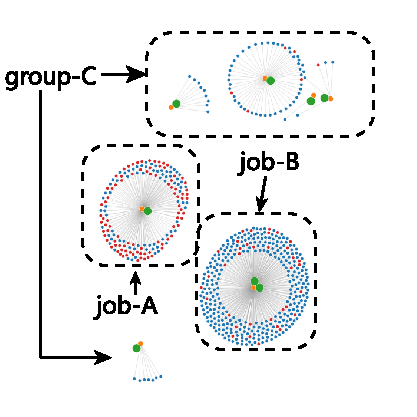
\includegraphics[height=0.57\textwidth]{2}
	\caption{主视图用例展示}
	\label{fig-6}
\end{figure}

图\ref{fig-6}是系统的主视图组件,它能够反映导致分布式系统中服务器节点负载过高的可疑作业,同时,它是Level-2组件的入口视图。如图所示,在时间戳114550处处理了八个作业单元和七个作业集群(绿色节点表示作业,橙色节点表示任务),并且每个作业仅具有一个子任务。我们可以看到每个任务节点下的蓝点都有多个实例节点。同时,处理红色实例节点的服务器机器表示此刻的高负载状态。据我们所知,作业调度程序将每个作业请求安排到几个不同的服务器计算机中,换句话说,每台计算机上运行的实例不少于一个。因此,我们无法将红色高负载实例节点包围的作业节点判断为导致服务器机器异常状态的可疑作业节点,如图5所示的作业-B。作业-B集群有多个服务器处于高负载状态的机器处理其任务实例。由于红色节点数量相对较少,我们可以估计作业-B不是客户发送的不合理请求。在这里,我们提出了一个新概念:高负载相关系数(HLCC)\footnote{High Load Correlation Coefficient},它表示中央作业与运行作业调度程序调度的实例的高负载机器之间的相关性。 HLCC可以通过以下算法计算:

$$HLCC=\frac{N_{ab}}{N}$$

如上面的算法所示,N表示作业总数的实例数。 Nab表示处理实例的异常服务器计算机的数量。在这种情况下,我们可以理解作业-A的HLCC为90/168(0.536)的可疑作业的定义,几乎是作业-B 36/220(0.164)的HLCC的三倍。组C充满了正常的作业集群,几乎没有高负载状态的节点。设置此控制组的含义是说明作业-A最有可能导致此时运行实例的几乎每个服务器节点都出现异常状态,同时,作业-B是一个很好的健康请求。客户。虽然有几个红色环绕的异常节点,但它无法描述作业-B是可疑的异常作业。很可能所有高负载服务器节点都是由服务器正在处理的任何其他任务实例引起的,或者服务器本身的硬件性能较差。因此,我们完成了从服务器到用户的异常映射。但是,由于实际存在正常的样本作业,我们不能得出结论是在客户请求高峰期间导致异常的环境问题。

\begin{figure}[h]
	\centering
	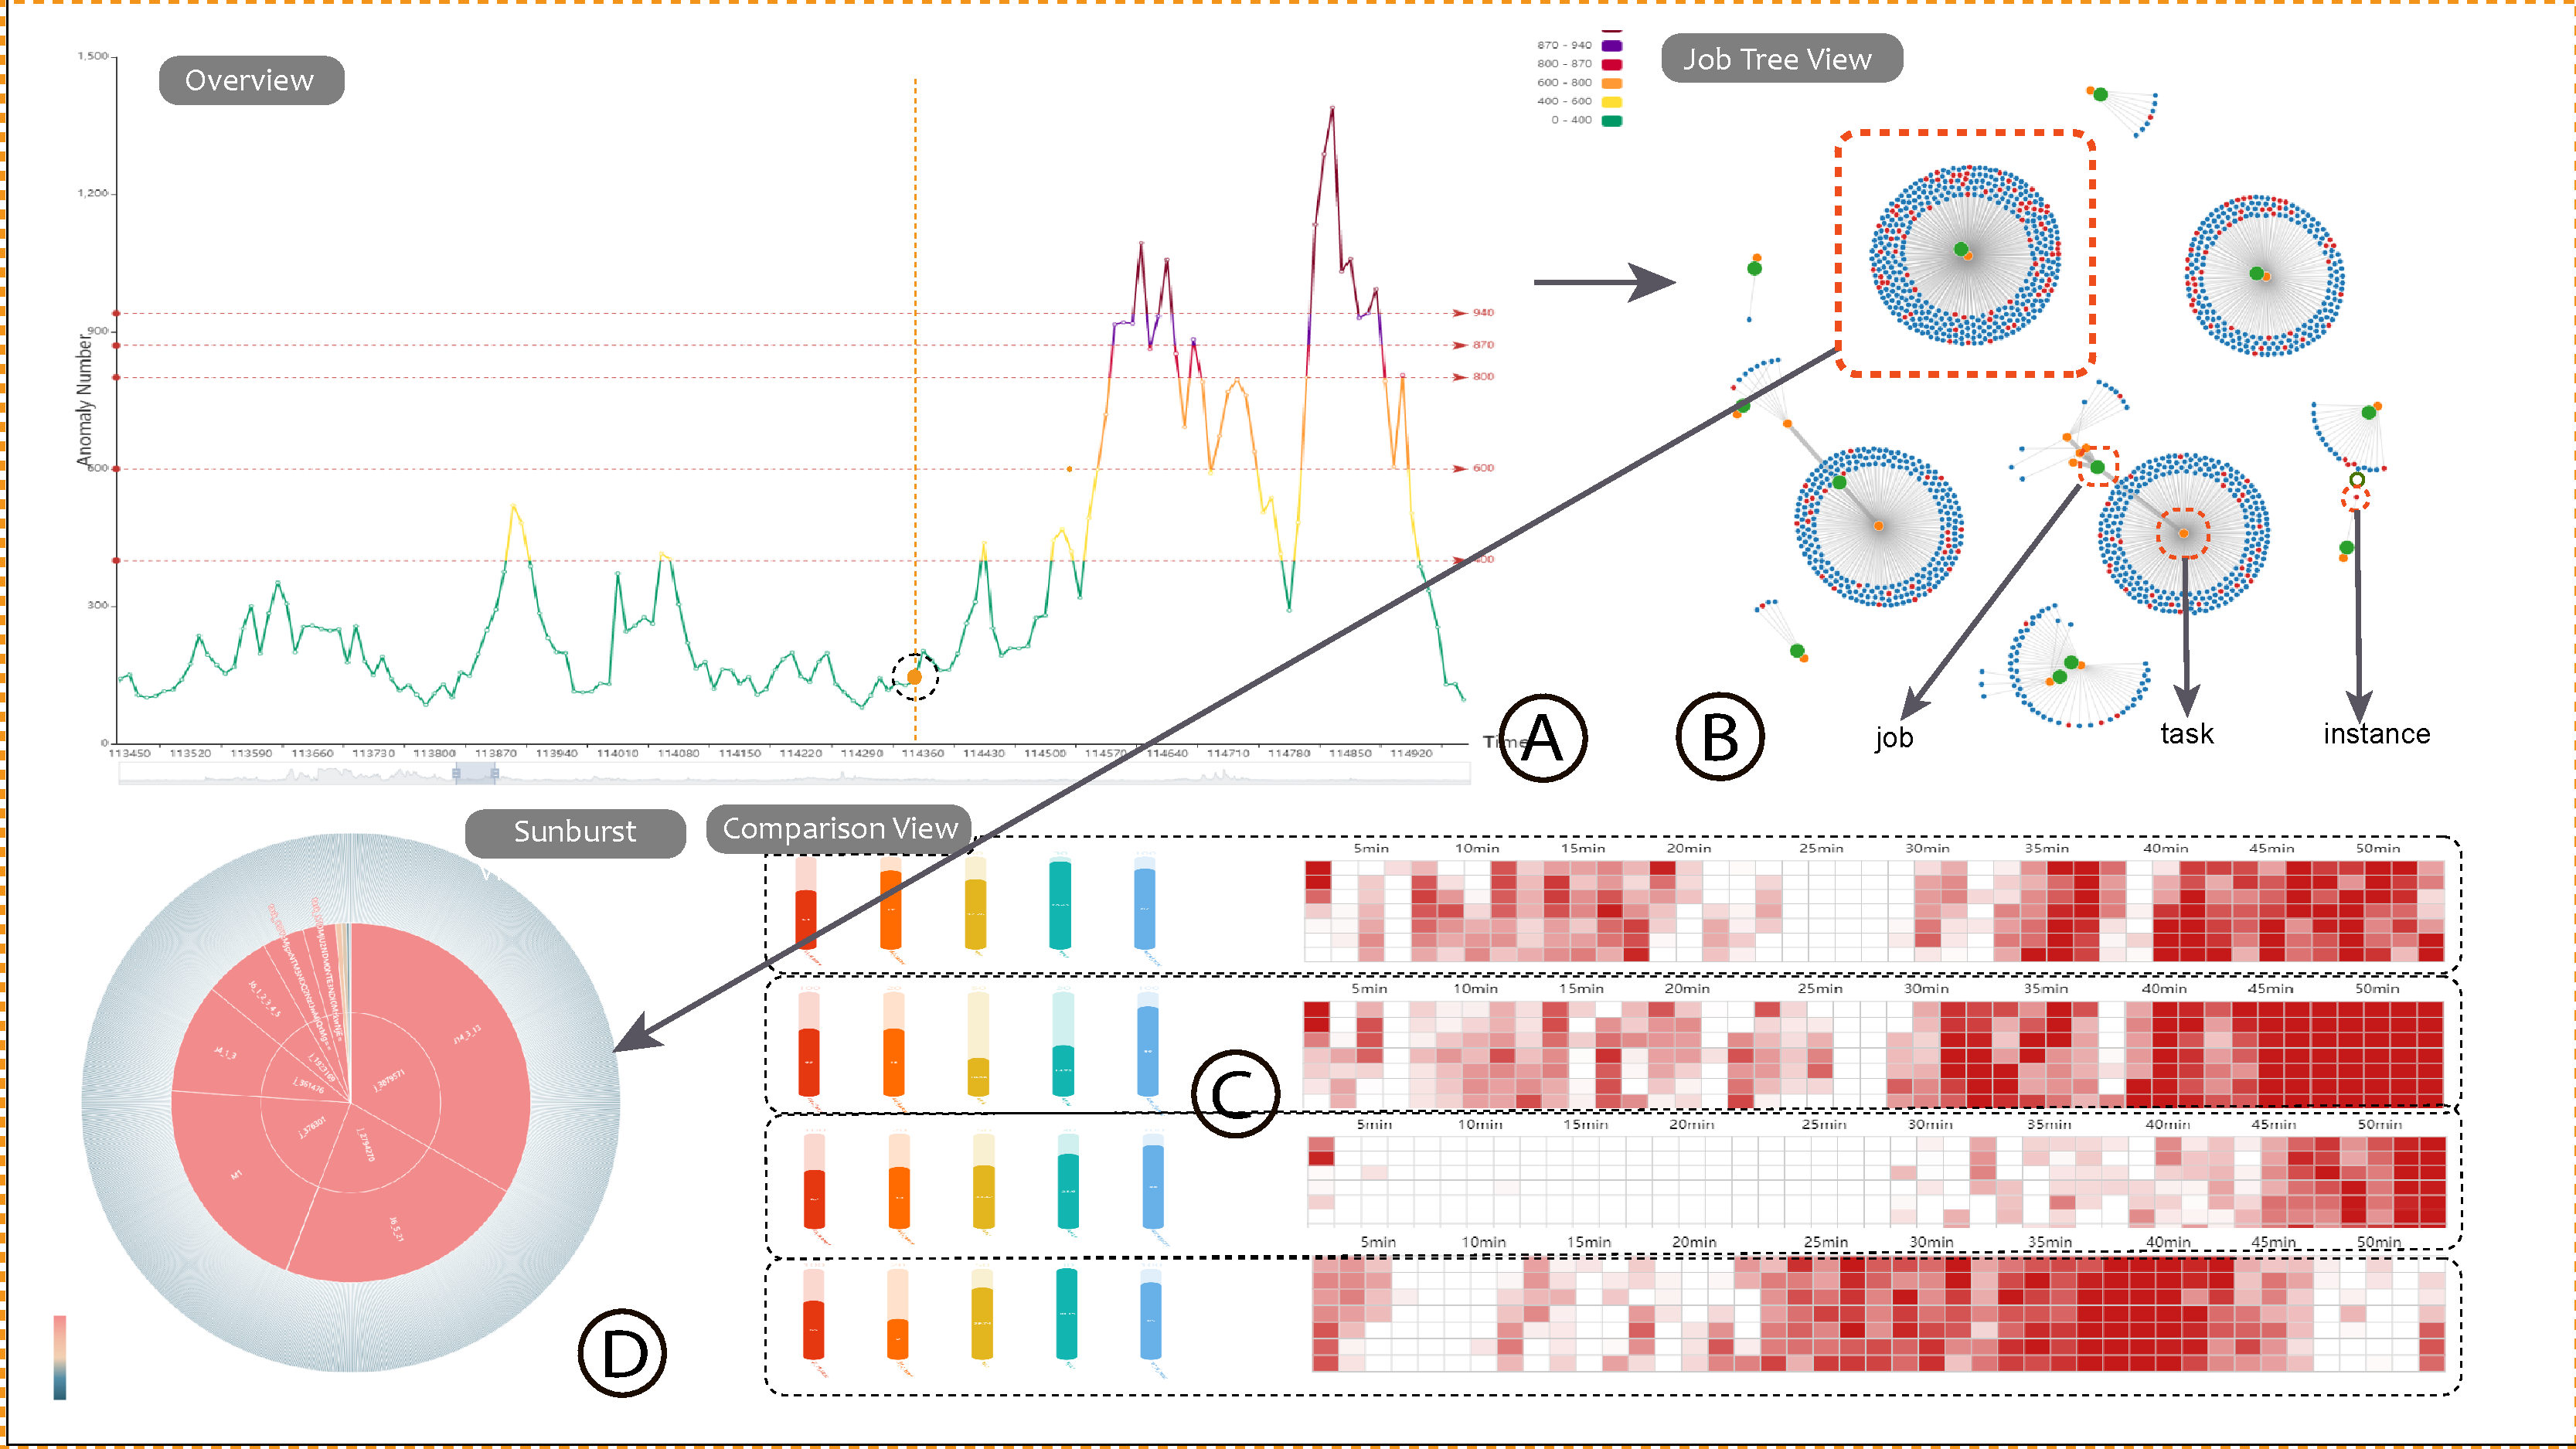
\includegraphics[width=0.95\textwidth]{00}
	\caption{系统屏幕截图}
	\label{fig-7}
\end{figure}

图\ref{fig-7}是JobPlot在时间戳114550的屏幕截图。在本节中,我们将通过模拟操作来说明JobPlot的工作过程。作为JobPlot的入口组件,区域A向操作员显示高负载服务器数量的分布。例如,我们可以看到价值从113450到114500维持在400以下的稳定水平,并从那时开始急剧上升至1000。时间戳控制条使得可以通过有限的时间线在大量时间戳下观察状态。我们选择A中的典型时刻114550,然后根据我们选择的时间刷新区域B作业树视图。如上所述,除了作业A之外,图中的所有作业集群都在稳定运行,其中HLCC远远高于视图中的任何其他作业集群。虽然其他工作的HLCC不为零,但其值在可接受的范围内,我们可以得出结论,中央作业节点不是导致这些服务器异常的原因。

区域D是与区域B在同一时间戳上的作业计划分布的旭日视图。如图所示,在旭日视图中记录了11个作业集群,其能够直观地显示作业集群的数量和比例。操作员可以通过交互事件查看单个作业或任务下的实例的整体分布,同时可以观察有关作业调度分布的详细信息。所有这些特征使得与比较视图组件交互更加合理和实用,如区域C所示。

从上述三个视图中,我们全面了解了大规模分布式系统中所有服务器的状态以及值得关注的服务器节点。作为单个节点的视图组件,区域C描绘了运行的关键参数和时间序列中的节点状态的直观显示。

区域C中的条形表示从左到右的CPU利用率,磁盘利用率,传入网络包的数量,传出网络包的数量以及所选服务器计算机的内存利用率。日历图表位于条形图的左侧,它反映了过去每十秒钟服务器节点的状态记录(每个块代表十秒)。根据视觉映射,红色越深,饱和度越大,节点的负载越高。

如区域C所示,比较视图的主体中有四个单独的模块。 C1和C2模块表示在区域B中的圆圈作业下的高负载中的两个服务器,C3和C4模块是正常服务器机器的跟踪记录。因此,我们完成了执行请求的服务器的综合时间序列描述。正如我们所料,高负荷组中节点的整体运行状态不如对比组的状态好,其中红色的块比直觉上的前两个模块更少且更稀疏。同时,条形图的值也小于高负荷值。

通过这种观察方式,时间序列视图可以全面地找出过去一小时内的高负荷异常时期。无论处理指令的服务器是否处于高负载状态,似乎30分钟后的时间戳是常见的异常时段。因此,我们可以看到分布式系统中的服务器在过去30分钟内出现异常峰值,这可能是由用户的峰值使用时间或某些因素(如该地区的电压或天气状况)引起的。

幸运的是,还有另一个证据证实了我们的视觉设计。 观察到的作业集群从时间戳114510开始追踪并持续近80秒。 可以在C1和C2模块中检查时刻114510,包括从114510到114550(当前)的深红色的四个块。 结果,服务器异常的时刻与作业被安排执行执行请求的时间完全相同。 这是一个有价值的发现,用于说明我们提出的HLCC数量确实合理且可以解释。